% ARINC 429 topologias

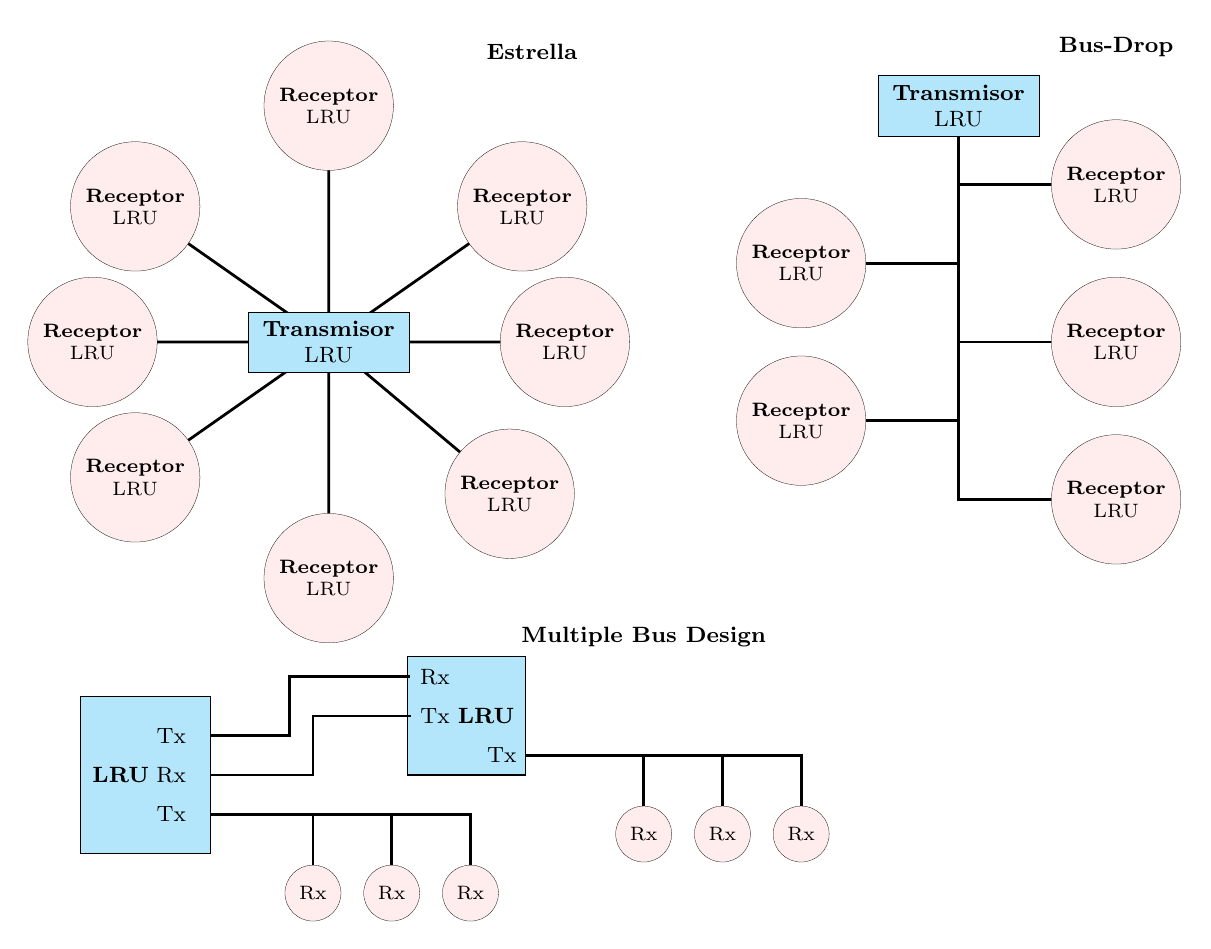
\begin{tikzpicture}[node distance=1cm, 
				font = \footnotesize , 
               Transmisor/.style ={ fill=cyan!30 , 
                          draw,
                          line width= 0.1 , 
						text width=1.8cm,
						align = center
                        } ,
               Receptor/.style ={  font = \scriptsize, 
						circle ,
                          fill=pink!30 , 
                          draw,
%						text width=1.2cm,
						align = center ,
                          line width= 0.1 , 
                        } ,
			]

% grilla
%  \draw[ green!50!black] (0,0) grid (20,10) ;

\path (3.5 , 7.5) coordinate (TxEstrella)
             (11.5 , 10.5) coordinate (TxBusDrop)
      ;

% Topologia estrella

\draw (TxEstrella) + (55:4.5) node {\bf Estrella};
\draw[line width=1]
               (TxEstrella) node[Transmisor]  {{\bf Transmisor} \\ LRU }
               -- +(0:3.0) node[Receptor]  {{\bf Receptor} \\ LRU }
(TxEstrella)  --  +(35:3.0) node[Receptor]  {{\bf Receptor} \\ LRU }
(TxEstrella)  --   +(90:3.0) node[Receptor]  {{\bf Receptor} \\ LRU }
(TxEstrella)  --   +(145:3.0) node[Receptor]  {{\bf Receptor} \\ LRU }
(TxEstrella)  --  +(180:3.0) node[Receptor]  {{\bf Receptor} \\ LRU }
(TxEstrella)  --   +(215:3.0) node[Receptor]  {{\bf Receptor} \\ LRU }
(TxEstrella)  --    +(270:3.0) node[Receptor]  {{\bf Receptor} \\ LRU }
(TxEstrella)  --    +(320:3.0) node[Receptor]  {{\bf Receptor} \\ LRU }
  ;

% Topologia estrella
\draw (TxBusDrop)  +(2,0.75)  node {\bf  Bus-Drop};
\draw[line width=1]
               (TxBusDrop) node[Transmisor]  {{\bf Transmisor} \\ LRU }
				         |- +(2,-1) node[Receptor]  {{\bf Receptor} \\ LRU }
(TxBusDrop) |- +(-2,-2) node[Receptor]  {{\bf Receptor} \\ LRU }
(TxBusDrop) |- +(2,-3) node[Receptor]  {{\bf Receptor} \\ LRU }
(TxBusDrop) |- +(-2,-4) node[Receptor]  {{\bf Receptor} \\ LRU }
(TxBusDrop) |- +(2,-5) node[Receptor]  {{\bf Receptor} \\ LRU }
;

% Topologia Multiple Bus Design

\draw [fill=cyan!30] (0.35,1) rectangle (2,3) 
	(1,2) node[text width=1cm] {\bf LRU}
		+ (0.5,0.5) node (Tx1) {Tx}
		+ (0.5,0.0) node (Rx1) {Rx}
		+ (0.5,-0.5) node (Tx11) {Tx}
;

\draw [fill=cyan!30] (4.5,2) rectangle (6,3.5) 
	(5.5,2.75) node {\bf LRU} +(2.0 , 1.0) node {\bf Multiple Bus Design}
		+ (-0.65,0.5) node (Rx2) {Rx}
		+ (-0.65,0.0) node (Tx2) {Tx}
		+ (0.2,-0.5) node (Tx22) {Tx}
;

\draw[line width=1] (Tx1) +(0.5 , 0) -- +(1.5,0) |- (Rx2) ;
\draw[line width=1] (Rx1) +(0.5 , 0) -- +(1.8,0) |- (Tx2) ;
\draw[line width=1] (Tx11) +(0.5 , 0) -- +(1.8,0) -- +(1.8 , - 1) node[Receptor] {Rx} ;
\draw[line width=1] (Tx11) +(0.5 , 0) -- +(2.8,0) -- +(2.8 , - 1) node[Receptor] {Rx} ;
\draw[line width=1] (Tx11) +(0.5 , 0) -- +(3.8,0) -- +(3.8 , - 1) node[Receptor] {Rx} ;

\draw[line width=1] (Tx22) +(0.3 , 0) -- +(1.8,0) -- +(1.8 , - 1) node[Receptor] {Rx} ;
\draw[line width=1] (Tx22) +(0.3 , 0) -- +(2.8,0) -- +(2.8 , - 1) node[Receptor] {Rx} ;
\draw[line width=1] (Tx22) +(0.3 , 0) -- +(3.8,0) -- +(3.8 , - 1) node[Receptor] {Rx} ;



\end{tikzpicture} 